\documentclass[a4paper,UTF8]{article}
\usepackage{ctex}
\usepackage[margin=1.25in]{geometry}
\usepackage{color}
\usepackage{graphicx}
\usepackage{amssymb}
\usepackage{amsmath}
\usepackage{amsthm}
\usepackage{listings}
\usepackage{color}
\usepackage{caption}
\usepackage{float}
\usepackage{subcaption}
%\usepackage[thmmarks, amsmath, thref]{ntheorem}
\definecolor{dkgreen}{rgb}{0,0.6,0}
\definecolor{gray}{rgb}{0.5,0.5,0.5}
\definecolor{mauve}{rgb}{0.58,0,0.82}

\lstset{frame=tb,
  language=bash,
  aboveskip=3mm,
  belowskip=3mm,
  showstringspaces=false,
  columns=flexible,
  basicstyle={\small\ttfamily},
  numbers=none,
  numberstyle=\tiny\color{gray},
  keywordstyle=\color{blue},
  commentstyle=\color{dkgreen},
  stringstyle=\color{mauve},
  breaklines=true,
  breakatwhitespace=true,
  tabsize=3
}

\theoremstyle{definition}
\newtheorem*{solution}{Solution}
\newtheorem*{prove}{Proof}
\usepackage{multirow}
\usepackage{url}
\usepackage[colorlinks,urlcolor=blue]{hyperref}
\usepackage{enumerate}
\renewcommand\refname{参考文献}


%--

%--
\begin{document}
\title{\textbf{《机器学习导论》赛题三报告}}
\author{181240035,刘春旭,\href{mailto:181240035@smail.nju.edu.cn}{181240035@smail.nju.edu.cn}}
\maketitle

\section{队伍得分与排名}
队伍名称为Chauncey10,共1171支队伍参加,排名为277.
截图如下:
\begin{figure}[h]
  \centering
  \begin{subfigure}[b]{0.45\textwidth}
      \centering
      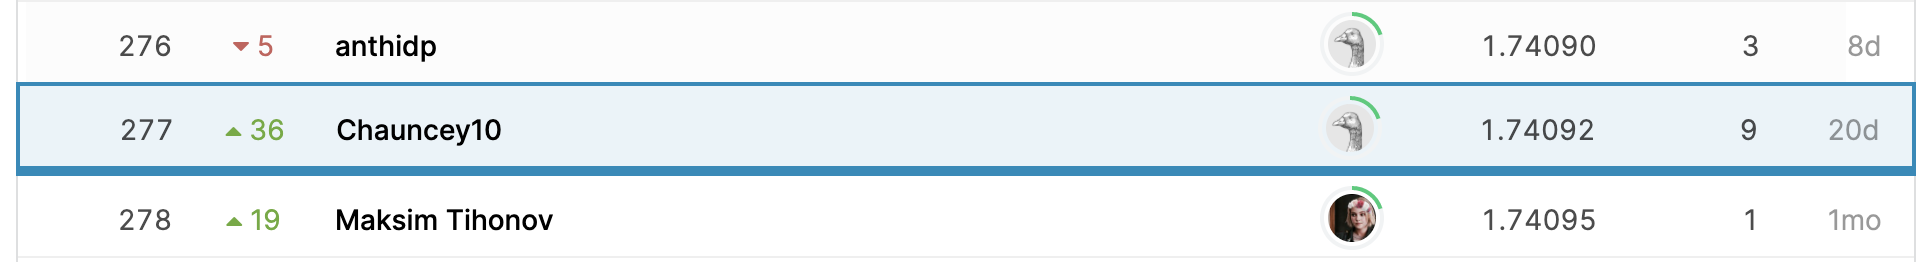
\includegraphics[width=\textwidth]{rank.png}
      \caption{排名}
  \end{subfigure}
  \hfill
  \begin{subfigure}[b]{0.45\textwidth}
      \centering
      
\includegraphics[width=\textwidth]{total.png}
      \caption{队伍总数}
  \end{subfigure}
  \caption{Private Leaderboard}
  \label{demo}
\end{figure}

\section{建模思路与方法}
使用Amazon开发出的\href{https://auto.gluon.ai/stable/index.html}{Autogluon}完成此次的实验,这是一个自动调参、挑选模型的AutoML包,完成本次竞赛全部代码量仅11行. 项目地址位于\href{https://github.com/lcxrocks/Kaggele_2021_Jun}{这里}下面进行详细说明:
\subsection{模型训练}
以下部分可以让Autogluon进行自主训练
\begin{lstlisting}
    from autogluon.tabular import TabularDataset, TabularPredictor
    import numpy as np
    import pandas as pd
    # 导入必要的包
    
    train_data = TabularDataset('train.csv')
    id, label = 'id', 'target'
    # 获得训练数据
    
    metric = 'log_loss'  # 使用log loss作为评估指标
    predictor = TabularPredictor(label=label, eval_metric=metric).fit(train_data.drop(columns=[id]),  presets='best_quality')  # 定义模型训练参数并开始训练
\end{lstlisting}
训练好的模型参数会储存在当前文件夹中,但是因为该文件夹大小过于巨大(44GB),故本次试验只上传了代码。

\subsection{模型预测}
通过以下代码生成提交文件(submission.csv)
\begin{lstlisting}
test_data = TabularDataset('test.csv')  # 导入测试数据集
preds = predictor.predict_proba(test_data.drop(columns=[id]), as_pandas=True)  # 开始训练模型
preds.insert(0, id, test_data[id])
preds.to_csv('submission.csv', index=False)  # 生成预测结果
\end{lstlisting}

\end{document}